\label{sec:eval}

This section evaluates \system’s impact on (i) wire payload size, (ii) time-to-first-rows (TTFR) for streaming, (iii) end-to-end transport latency on a real NL2SQL benchmark workload with fixed SQL, and (iv) codec trade-offs within Parquet. Full recorded runs and reproduction commands are included in the project artifacts.

\subsection{Experimental setup}
\noindent\textbf{Server and protocols.}
We run a local MCP server that exposes a JSON-RPC control plane and an HTTP data plane. The baseline arm returns tabular tool outputs as JSON records through MCP. The enhanced arm returns a descriptor through MCP and delivers the bytes via HTTP as either a Parquet blob or a length-prefixed Parquet chunk stream; it may additionally call \texttt{describe\_result\_formats} to obtain size hints, unless using one-shot server-side selection.

\smallskip
\noindent\textbf{Datasets.}
We use (i) synthetic grids with controlled \((n\_rows, n\_cols)\), (ii) TPC-DS \texttt{catalog\_sales} slices to characterize format scaling and decode proxies, and (iii) BIRD dev query results (SQLite port) to evaluate transport on real workloads while controlling for NL2SQL.

\smallskip
\noindent\textbf{Metrics.}
We report \textbf{bytes} (payload size on the wire), \textbf{fetch latency} (baseline JSON fetch vs.\ enhanced single fetch), \textbf{describe+fetch latency} (client-driven selection overhead), and a TTFR proxy for streaming using first-chunk bytes and time-to-first-chunk decode. On BIRD we emphasize p95 and \textbf{aggregate sums of bytes} across the split, since median results are often tiny.

\subsection{Format size scaling on TPC-DS slices}
Figure~\ref{fig:tpcdsSizeScaling} shows payload bytes as a function of rows for representative column counts. Parquet consistently yields the smallest wire sizes, while Arrow IPC is intermediate and JSON is largest. This behavior matches the expected inefficiency of JSON for tabular layouts (repeated keys, string overhead), and it motivates keeping large tables out of MCP message bodies.

\begin{figure}[t]
  \centering
  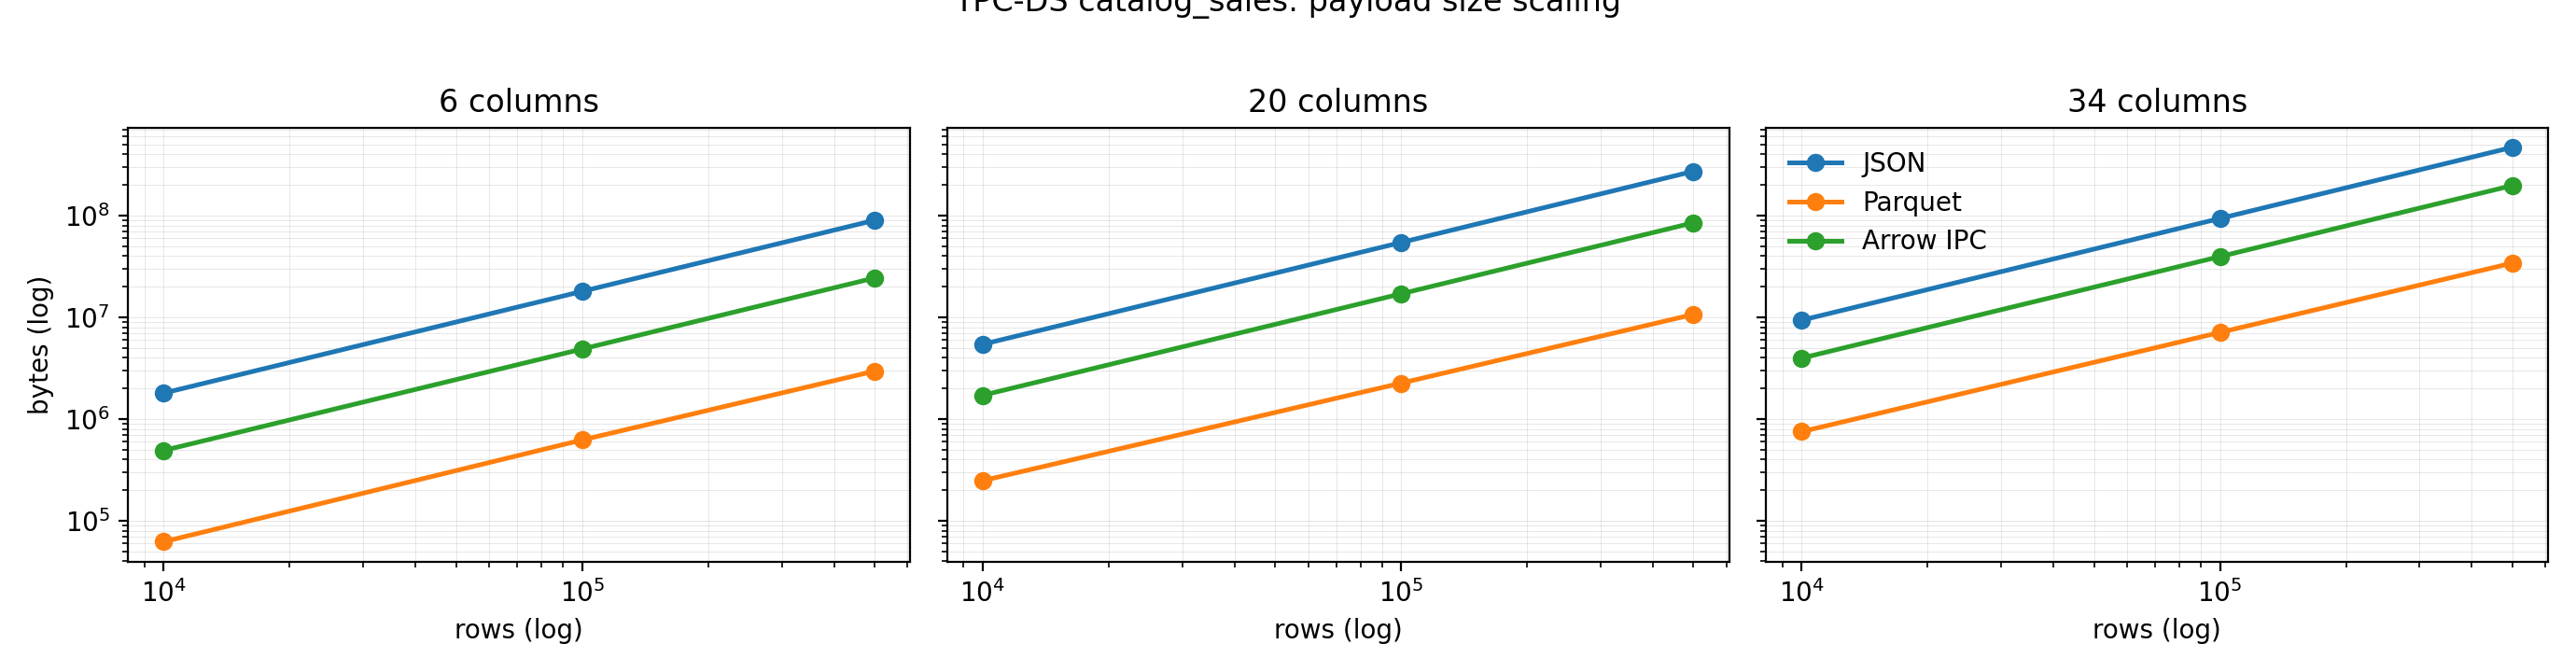
\includegraphics[width=\columnwidth]{figures/fig_A1_tpcds_size_scaling.png}
  \Description{Log-scale line plots showing how payload bytes scale with row count for JSON, Parquet, and Arrow IPC under three column projections. Parquet is consistently smallest; JSON is largest.}
  \caption{TPC-DS \texttt{catalog\_sales}: payload size scaling for JSON vs.\ Parquet vs.\ Arrow IPC across row counts and column projections.}
  \label{fig:tpcdsSizeScaling}
\end{figure}

\subsection{Streaming and time-to-first-rows}
Chunk streaming improves responsiveness when the client can begin processing before receiving the full result. Figure~\ref{fig:firstChunkVsTotal} plots first-chunk size versus total size for Parquet and Arrow IPC streams. For large results, first-chunk bytes are a small fraction of total bytes, enabling low TTFR and supporting early termination when an agent has sufficient evidence to proceed.

\begin{figure}[t]
  \centering
  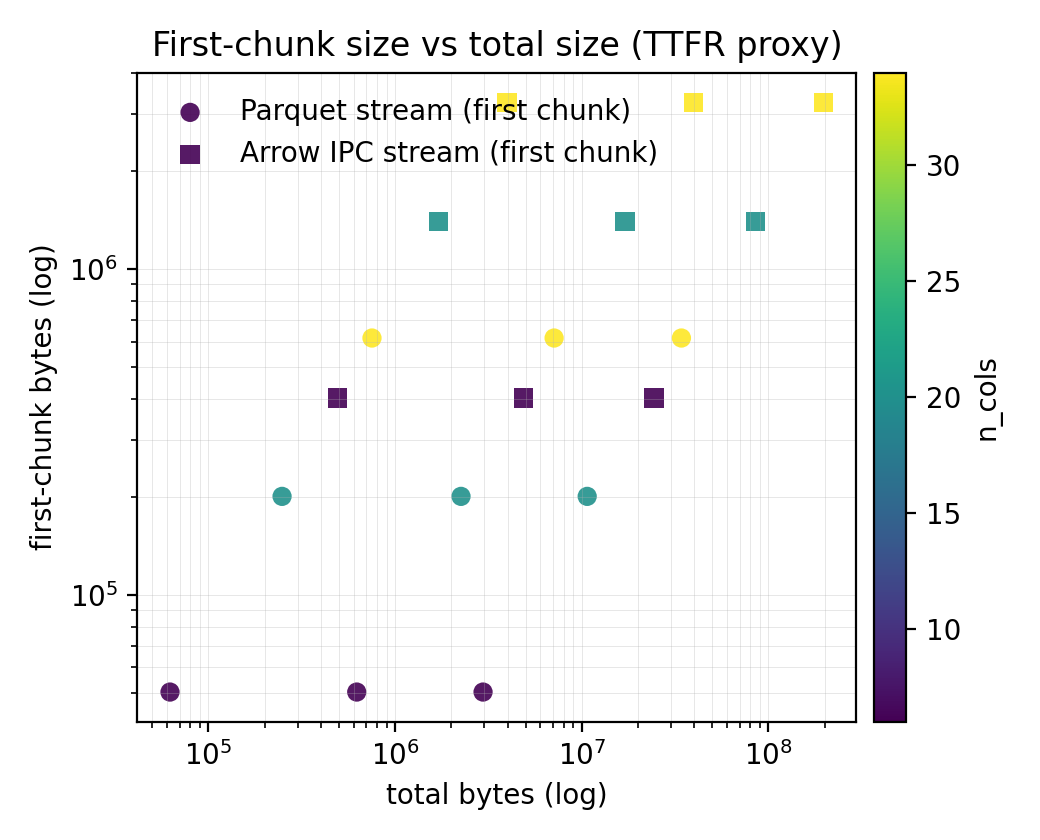
\includegraphics[width=\columnwidth]{figures/fig_A2_tpcds_first_chunk_bytes.png}
  \Description{Scatter plot of first-chunk bytes versus total bytes for Parquet and Arrow IPC streaming, with color indicating column count. First chunks are much smaller than totals for large payloads.}
  \caption{TTFR proxy: first-chunk bytes vs.\ total bytes for streaming formats. Smaller first chunks enable faster time-to-first-rows and early-stop behaviors.}
  \label{fig:firstChunkVsTotal}
\end{figure}

\subsection{Decode proxy calibration}
To support \texttt{min\_latency} selection beyond pure ``min bytes'', we calibrate a simple decode proxy: nanoseconds per byte for decoding representative payloads. Figure~\ref{fig:decodeProxy} shows median decode ns/byte (IQR) for JSON, Parquet blob, and Arrow IPC blob on TPC-DS slices. As expected, Arrow IPC decodes substantially faster in Arrow-native stacks, while Parquet trades some decode cost for wire size.

\begin{figure}[t]
  \centering
  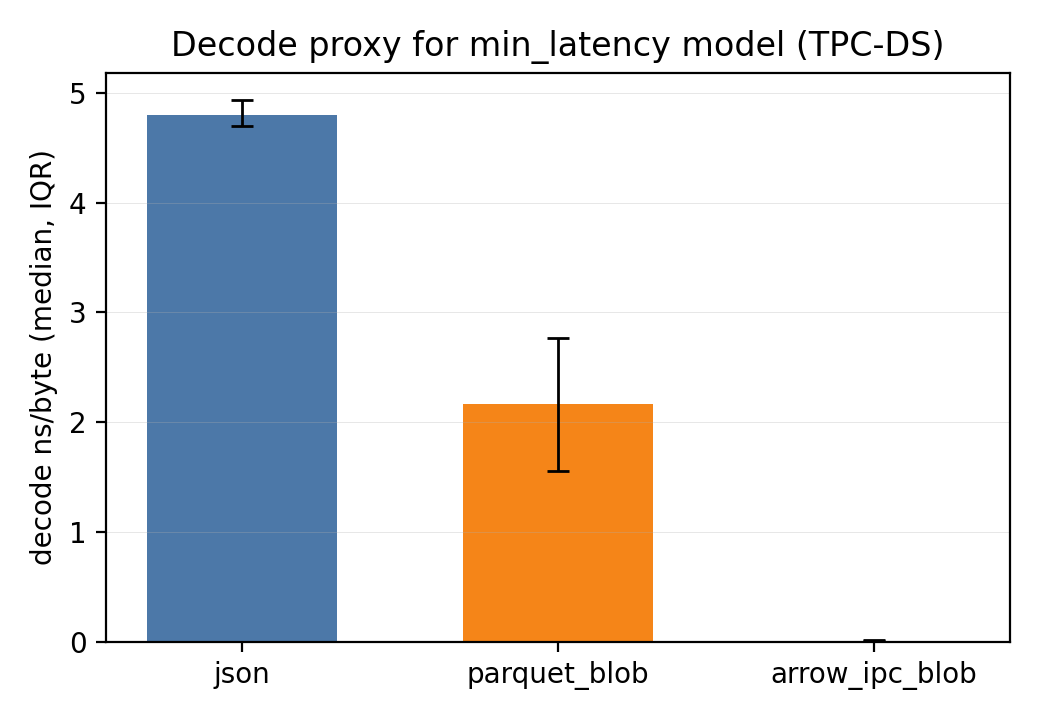
\includegraphics[width=0.85\columnwidth]{figures/fig_A3_tpcds_decode_ns_per_byte.png}
  \Description{Bar chart of decode nanoseconds per byte (median with IQR) for JSON, Parquet blob, and Arrow IPC blob. Arrow IPC shows near-zero decode cost per byte compared to the others.}
  \caption{Decode proxy calibration (TPC-DS): median decode ns/byte (IQR) for JSON, Parquet, and Arrow IPC. Used as an optional term in \texttt{min\_latency} scoring.}
  \label{fig:decodeProxy}
\end{figure}

\subsection{BIRD transport: bytes and latency on real workloads}
We evaluate \system on BIRD dev with \textbf{gold SQL} to isolate transport effects from NL2SQL quality. For each question, the client executes the reference SQL on the corresponding SQLite database, registers the materialized result once, and then compares two transport arms on the same result: (A) baseline ``JSON-only'' MCP delivery, and (B) enhanced delivery with hint-aware format choice and Parquet blob fetch when beneficial.

\smallskip
\noindent\textbf{Payload (wire bytes).}
On BIRD full dev (1534 queries), the aggregate wire volume decreases from 43{,}439{,}928 bytes (baseline JSON) to 6{,}386{,}514 bytes (enhanced selection), a 6.8$\times$ reduction. Medians remain small (57 bytes) because many queries return tiny results; p95 bytes decreases from 11{,}966 to 3{,}650, and the enhanced arm chooses Parquet for 164/1534 queries, concentrating savings on the tail.

\smallskip
\noindent\textbf{Latency and overhead.}
Figure~\ref{fig:birdLatencyPaired} plots per-query variant latency against baseline latency (paired). On localhost, the enhanced \emph{single fetch} remains comparable to baseline fetch because the dominant effect is network loopback; the primary overhead is the additional ``describe'' call in client-driven selection. Figure~\ref{fig:birdOverheadBreakdown} breaks down median overhead, highlighting that one-shot server-side selection can remove the describe round-trip while retaining the data-plane benefits.

\begin{figure}[t]
  \centering
  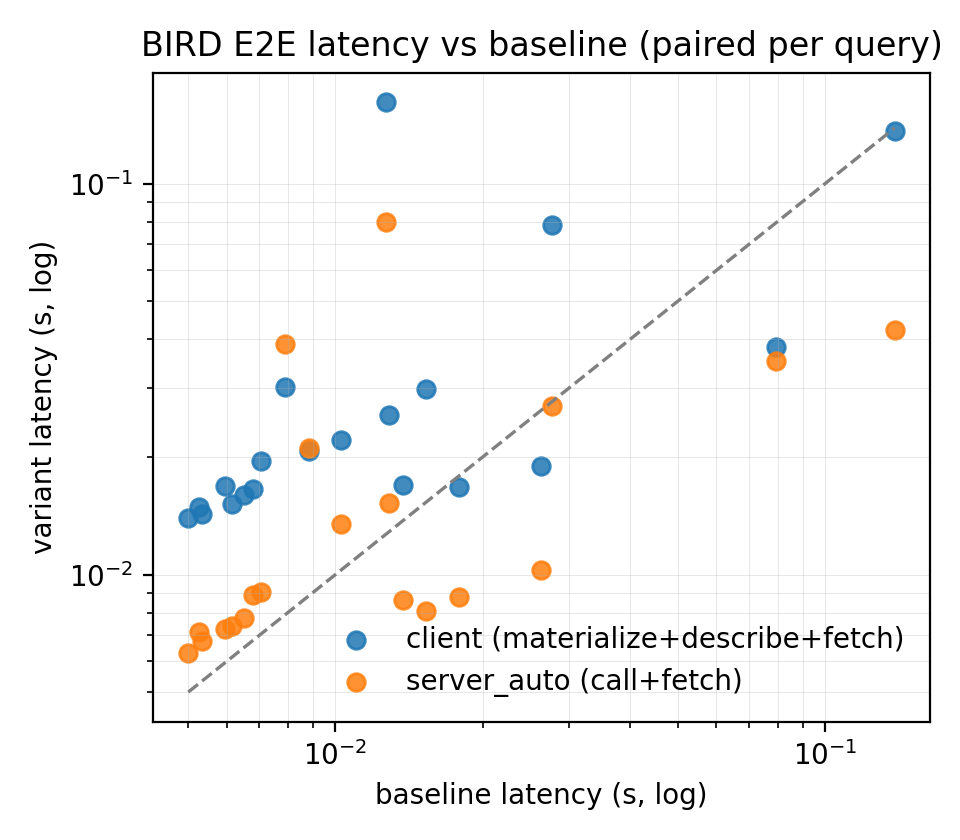
\includegraphics[width=\columnwidth]{figures/fig_B1_bird_latency_paired.png}
  \Description{Paired scatter plot on log-log axes comparing per-query variant latency against baseline latency for client selection and server-side auto selection. A diagonal reference line indicates parity.}
  \caption{BIRD paired per-query latency: client-driven selection (materialize+describe+fetch) and one-shot server-side selection (call+fetch) compared to baseline (JSON fetch). Both axes are log-scaled seconds.}
  \label{fig:birdLatencyPaired}
\end{figure}

\begin{figure}[t]
  \centering
  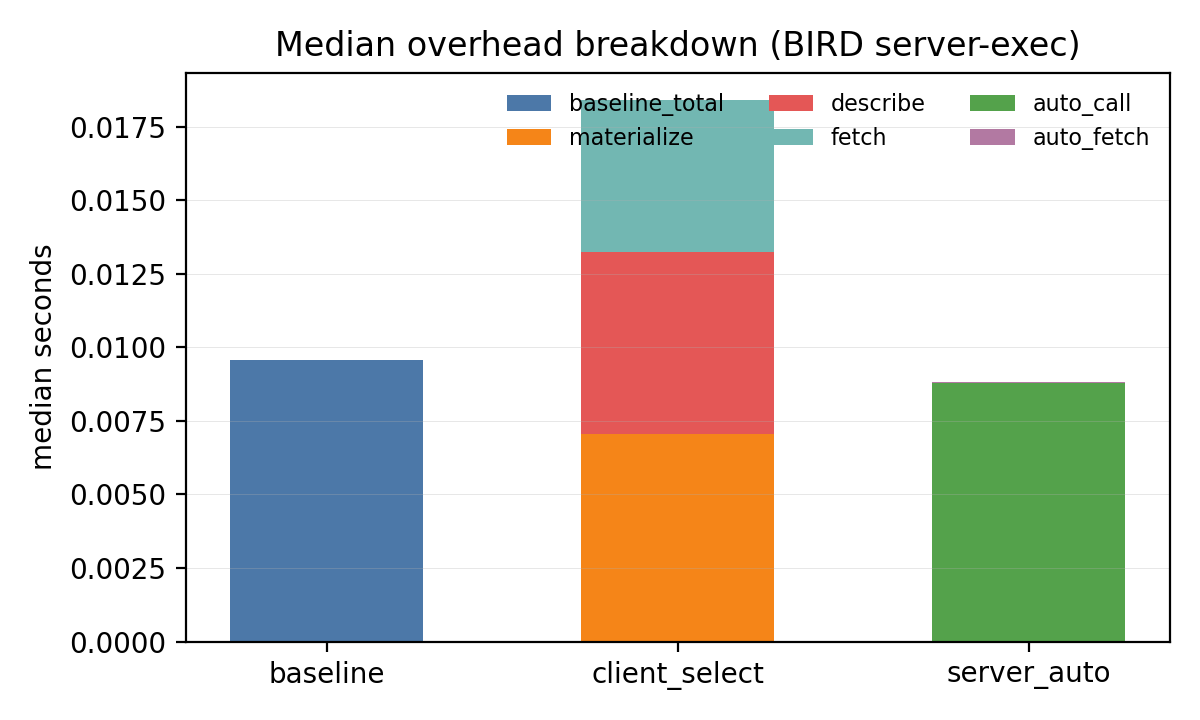
\includegraphics[width=\columnwidth]{figures/fig_B3_bird_overhead_breakdown.png}
  \Description{Stacked bar chart breaking down median overhead in seconds for baseline, client selection, and server auto. Client selection includes materialize, describe, and fetch components.}
  \caption{Median overhead breakdown on BIRD: baseline total vs.\ client selection (materialize, describe, fetch) vs.\ server-side one-shot selection.}
  \label{fig:birdOverheadBreakdown}
\end{figure}

\subsection{Codec/encoding trade-offs within Parquet}
Within the Parquet arm, codec choice trades off wire size against encode+decode time. Figure~\ref{fig:codecBytes} shows Parquet bytes for a representative TPC-DS-derived table under different codec/strategy settings. Figure~\ref{fig:codecTradeoff} plots encode+decode time versus bytes, illustrating a Pareto frontier: Zstd often reduces bytes more than Snappy at moderate CPU cost, while Gzip tends to be slower for similar or smaller gains.

\begin{figure}[t]
  \centering
  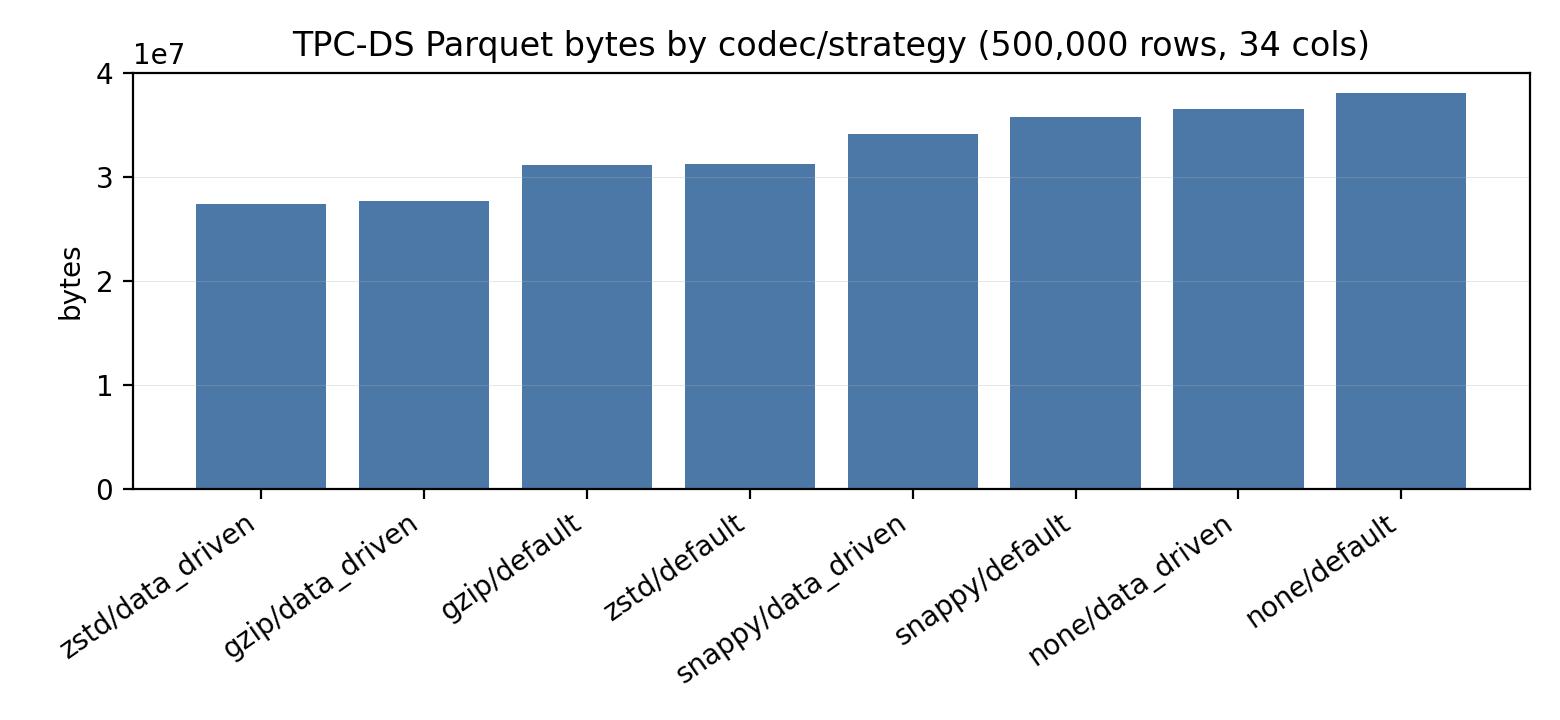
\includegraphics[width=\columnwidth]{figures/fig_C1_codec_bytes_bars.png}
  \Description{Bar chart comparing Parquet payload bytes across codec and encoding-strategy combinations for a fixed TPC-DS-derived table.}
  \caption{TPC-DS Parquet bytes by codec/strategy for a representative table.}
  \label{fig:codecBytes}
\end{figure}

\begin{figure}[t]
  \centering
  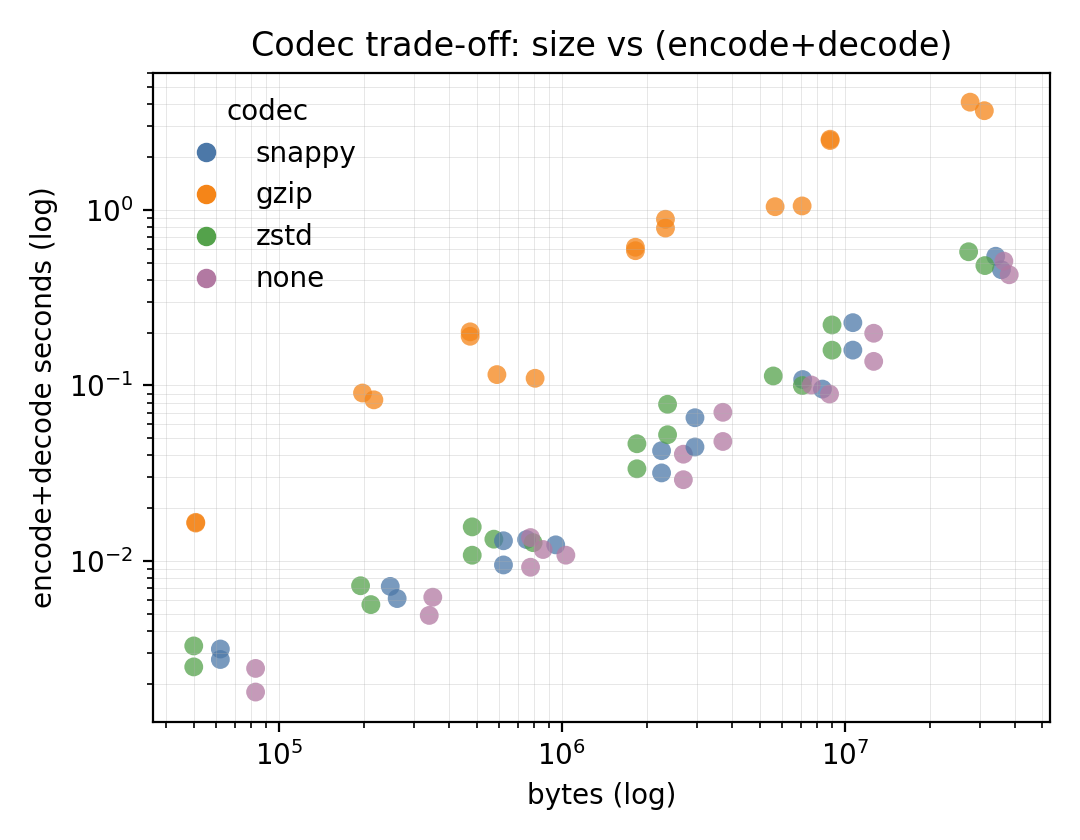
\includegraphics[width=\columnwidth]{figures/fig_C2_codec_tradeoff_scatter.png}
  \Description{Scatter plot on log-log axes showing encode+decode time versus payload bytes for multiple codecs. Points reveal size-latency trade-offs and a Pareto frontier.}
  \caption{Codec trade-off: payload size versus encode+decode time (log-log). Points illustrate the Pareto structure across codecs.}
  \label{fig:codecTradeoff}
\end{figure}

\subsection{Threats to validity}
\textbf{Localhost transport:} reported millisecond latencies reflect same-machine loopback and do not capture WAN RTT or bandwidth variability; payload ratios are more portable than absolute times. \textbf{Gold SQL isolation:} core BIRD runs execute reference SQL, isolating transport but not evaluating NL2SQL accuracy. \textbf{Result caps and caching:} benchmarks cap pathological result sizes and use pragmatic caching; we compare baseline and enhanced on the same materialized result ids to preserve fairness.